\documentclass[fleqn,12pt]{article}

\usepackage{float}


\usepackage[utf8]{inputenc}
\usepackage[dvips]{graphicx}
%\usepackage{a4wide}
\usepackage{epsfig}
\usepackage{fancybox}
\usepackage{verbatim}
\usepackage{array}
\usepackage{latexsym}
\usepackage{alltt}
\usepackage{amssymb}
\usepackage{amsmath}
\usepackage{enumerate}
%\usepackage{fullpage}
\usepackage{hyperref}
\usepackage{listings}
\usepackage{color}
\usepackage{algorithm}
\usepackage{algpseudocode}
\usepackage{textcomp}
\usepackage[hmargin=3cm,vmargin=5.0cm]{geometry}


%misc libraries goes here
\usepackage{tikz}
\usetikzlibrary{automata,positioning}

\lstset
{
    language=[LaTeX]TeX,
    breaklines=true,
    basicstyle=\tt\scriptsize,
    keywordstyle=\color{blue},
    identifierstyle=\color{magenta},
}

%\topmargin=0cm
\topmargin=-1.8cm
\addtolength{\textheight}{6.5cm}
\addtolength{\textwidth}{2.0cm}
%\setlength{\leftmargin}{-5cm}
\setlength{\oddsidemargin}{0.0cm}
\setlength{\evensidemargin}{0.0cm}

\newcommand{\HRule}{\rule{\linewidth}{1mm}}
\newcommand{\kutu}[2]{\framebox[#1mm]{\rule[-2mm]{0mm}{#2mm}}}
\newcommand{\gap}{ \\[1mm] }

\newcommand{\Q}{\raisebox{1.7pt}{$\scriptstyle\bigcirc$}}
\newcommand{\minus}{\scalebox{0.35}[1.0]{$-$}}


\begin{document}

\noindent
\HRule \\[3mm]
\small
\begin{tabular}[b]{lp{2.9cm}r}
{\epsfig{file=metulogo.eps,width=5mm}} Middle East Technical University &  &
{\epsfig{file=bmblogo.eps,width=5mm}} Department of Computer Engineering \\
\end{tabular} \\
\begin{center}

                 \LARGE \textbf{CENG 280} \\[4mm]
                 \Large Formal Languages and Abstract Machines \\[4mm]
                \normalsize Spring 2018-2019 \\
                    \Large Take Home Exam 3
\end{center}
\HRule

\begin{center}
Due date: May 22, 2019
\end{center}

\section*{Objectives}
To familiarize with computation using Turing Machines and inspect aspects of the class of languages associated with them.
\\

\section*{Specifications}

You must adhere to the notation conventions adopted in the textbook. Use the standard deterministic Turing Machine as defined in the book unless stated otherwise. You should utilize basic machines notation whenever asked for.
\\
\\
Your solution should be delivered as a \texttt{pdf} file generated using the \texttt{tex} template provided or employing other text editors. You are allowed to use only text and vector images in your submission, i.e. use of raster images is clearly forbidden.
\\
\\
Questions and submission regulations are included in subsequent sections. Assume that any input string $w$ over a finite alphabet $\Sigma$ is initially placed on the tape of the standard TM always as $\triangleright\underline{\sqcup} w$ unless stated otherwise. If multi-tape TM is used then the same placement occurs on its first tape and initial configuration will be as $\triangleright\underline{\sqcup}$ concerning the remaining tapes. 
\\
\\
Designing your solutions to the tasks, explicitly state any assumptions you make and pay particular attention to the notation you use. Your proofs must be sound and complete. Grading will be heavily affected by the formalization of your solutions.

\newpage

\section*{Question 1 \hfill \normalfont{(12 pts)}}
Answer the questions using the following Turing Machine.
\\ \\
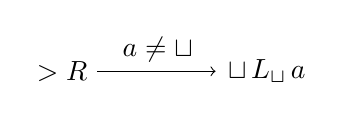
\begin{tikzpicture}[shorten >= 1pt, node distance=2cm, on grid, auto]
	\node (0) {$> R$};
	\node (1) [right=of 0, xshift=0.6cm] {$\sqcup\, L_{\sqcup}\, a$};

	\path[->]
		(0) edge node {$a\neq\sqcup$} (1);
\end{tikzpicture}

\paragraph{a.} Write the given TM in \textbf{five-tuple notation} as $M = (K, \Sigma, \delta, s, H)$ \textbf{explicitly} specifying each constituent. Let $\Sigma = \{a, b, \sqcup, \triangleright\}$ and $\delta(q, \triangleright) = (q, \rightarrow)$ for all $q \in K-H$. Denote $\delta$ as a \textbf{table}. \hfill \rlap{\hspace*{-3em}(6 pts)}
\paragraph{b.} Using M defined in \textbf{(a)}, write down the \textbf{computation} (sequence of configurations related by $\vdash_M$) for the following initial configurations. \hfill \normalfont{(6 pts)}
\begin{enumerate}[\bfseries(i)]
  \item $(s,\,\triangleright\sqcup\sqcup b\underline{a}b)$.
  \item $(s,\,\triangleright a\underline{a}a)$.
  \item $(s,\,\triangleright\underline{a}\sqcup b b)$.
\end{enumerate}
\noindent

\section*{Question 2 \hfill \normalfont{(8 pts)}}
Given the following Turing Machine on the alphabet $\Sigma=\{a, b, c, \sqcup, \triangleright\}$,
\\ \\
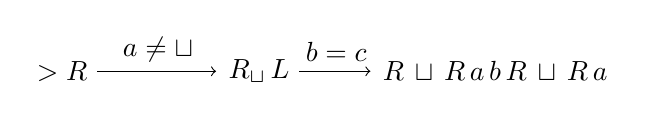
\begin{tikzpicture}[shorten >= 1pt, node distance=2cm, on grid, auto]
	\node (0) {$> R$};
	\node (1) [right=of 0, xshift=0.5cm] {$R_{\sqcup}\, L$};
	\node (2) [right=of 1, xshift=1cm] {$R\,\sqcup\,R\,a\,b\,R\,\sqcup \,R\, a$};

	\path[->]
		(0) edge node {$a\neq\sqcup$} (1)
		(1) edge node {$b = c$} (2);
\end{tikzpicture}
\\
\\
\textbf{trace} its operation on the input string $babc$ (intially placed on the tape as $\triangleright\underline{\sqcup} babc$) without explicitly referring to the particular set of states. In plain English, write down the set of \textbf{actions taken} by the TM upon encountering \textbf{any} string over $(\Sigma-\{\sqcup,\triangleright\})^*$ on its tape.
\noindent
\\
\section*{Question 3 \hfill \normalfont{(10 pts)}} 
Given the following Turing Machine $M$ on the alphabet $\Sigma=\{a, b, \#, \sqcup, \triangleright\}$, answer the questions.
\\ \\
\begin{tikzpicture}[shorten >= 1pt, node distance=2cm, on grid, auto]
	\node (6) {$> R$};
	\node (0) [right=of 0] {$R_{\overline{a}}$};
	\node (1) [right=of 0] {$R_{\overline{b}}$};
	\node (2) [below=of 1] {$L_{\sqcup}$};
	\node (3) [right=of 1] {$\#$};
	\node (4) [right=of 3] {$\,L_{\overline{b}}\, R\, a\, R_\# b$};
	\node (5) [right=of 4] {$R$};

	\path[->]
		(6) edge node {} (0)
		(6) edge [bend right] node {$\sqcup$} (2)
		(0) edge node {$b$} (1)
		(0) edge [bend right] node {$\sqcup$} (2)
		(1) edge node {$a$} (3)
		(1) edge node {$\sqcup$} (2)
		(3) edge node {} (4)
		(4) edge node {} (5)
		(5) edge [in=50, out=20, above] node {$b$} (1)
		(5) edge [in=-10, out=-20, above] node {$\sqcup$} (2)
		(5) edge [in=-60, out=-20, above] node {$a$} (3);
		%(4) edge [in=90, out=90] node [swap] {$1^1$} (5)
		%(6) edge node [swap] {$1^2$} (8)
		%(8) edge [in=70, out=10, loop] node {$1^2$} (8)
\end{tikzpicture}
\\
\paragraph{a.} Write the language $L$ over $\{a,b\}$ that $M$ \textbf{semidecides} using set notation. \hfill \normalfont{(5 pts)}
\paragraph{b.} Using \textbf{Definition 4.2.2} of the textbook, identify the function $f\,:\, \{a,b\}^*\mapsto\{a, b\}^*$ such that $M(w)=f(w)$ where $w\in\{a,b\}^*$. \hfill \normalfont{(5 pts)}


\section*{Question 4 \hfill \normalfont{(10 pts)}}
Using \textbf{basic machines notation}, construct a \textbf{multi-tape} Turing Machine that \textbf{decides} the following language:
\\\\
$L$ = $\{wcu\;:\; w, u \in\{a,b\}^*,\;w(2i) = w(2i-1) = u(i) \textrm{ for } i\,=\,1, ..., |u|\}$.
\noindent \\

\section*{Question 5 \hfill \normalfont{(10 pts)}}
Using \textbf{basic machines notation}, construct a \textbf{multi-tape} Turing Machine that \textbf{computes} the following function:
\\\\
$f\,:\,\{a,b\}^* \mapsto \{a,b\}^*$ where $f(u) = v$ such that 
\begin{flalign*}
&v(2i-1) = u(i)\\
&v(2i) = u(|u|-i-1)
\end{flalign*}
for $i\in\mathbb{N}$ within $\left[1, \left\lceil\dfrac {|u|} {2}\right\rceil\right]$.
\noindent \\ \\

\section*{Question 6 \hfill \normalfont{(12 pts + 10 pts bonus)}}
A variant of Turing Machine is the deterministic \textbf{queue TM} defined as a quintuple $(K, \Sigma, \delta, s, H)$ where $K$ is the set of states; $\Sigma$ is a finite alphabet containing $\triangleright$ to denote the left end of the queue; $s\in K$ is the initial state; $H\subseteq K$ is the set of final states; and $\delta\;:\;(K-H) \times \Sigma \mapsto K\times(\Sigma \cup \{\downarrow\})$ is the transition function where $\delta(q,a) = (p,X)$ for $p\in K-H$, $q\in K$, $a\in\Sigma$, $X\in\Sigma \cup \{\downarrow\}$ indicates that whenever the machine is at state $q$ and there is $a$ at the \textbf{front} position of the queue, the machine enters the state $p$ and takes the action $X$. If $X \in \Sigma$, the machine \textbf{enqueues} the element $X$ at the \textbf{rear} position of the queue. Otherwise if $X=\; \downarrow$, the machine \textbf{pops} the element at the front. Note that by these mechanisms the queue can get arbitrarily large or small.
\paragraph{a.} Impose restrictions on $\delta$ so that the pop operation is \textbf{not} allowed in an empty queue and enqueueing of $\triangleright$ \textbf{is} forbidden. \hfill \normalfont{(4 pts)}
\paragraph{b.} Add the flexibility of taking action \textbf{regardless of} what element is placed at the front of the queue, using $e$-transitions in $\delta$ in a way that \textbf{preserves} the determinism of the machine. Also update the sets over which $\delta$ is defined. \hfill \normalfont{(4 pts)}
\paragraph{c.} Define the \textbf{yields-in-one-step} relation of the machine, covering every case. \hfill \normalfont{(4 pts)}
\paragraph{d.} Construct a deterministic queue TM to \textbf{semidecide} the language $L =\{w^Rcw\;:\; w\in\{a,b\}^*\}$.  Your solution to this option will be considered as a bonus, provide a solution if you want to get extra points. You may invent your own graphical notation of the queue TM. \hfill \normalfont{(bonus: 10 pts)}

\pagebreak 

\section*{Question 7 \hfill \normalfont{(20 pts)}} 
Another variant of the Turing Machine can be defined as a deterministic TM where you can read the character at the \textbf{front} and \textbf{rear} positions of the input string on the tape, and perform \textbf{insertion} and \textbf{deletion} of cells \textbf{only} at the front and rear positions. Call this TM the \textbf{insert-delete TM} and assume that it does not have any additional functionality other than those mentioned. 
\paragraph{a.} Define the insert-delete TM as a \textbf{tuple}, stating the type of each constituent and identifying their functionalities. \hfill \normalfont{(5 pts)}
\paragraph{b.} Define the notion of \textbf{configuration} for the insert-delete TM. \hfill \normalfont{(2 pts)}
\paragraph{c.} Define the \textbf{yields-in-one-step} relation of the machine. Write in set notation the language \textbf{recognized} by the reflexive transitive closure of yields-in-one-step relation.  \hfill \rlap{\hspace*{-3em}(4 pts)}
\paragraph{d.} Prove that the insert-delete TM is \textbf{equivalent} to the standard TM. Write down how each case should be proved without going over every possible detail.\hfill \normalfont{(9 pts)}
\noindent \\\\

\section*{Question 8 \hfill \normalfont{(10 pts)}} 

Construct an \textbf{unrestricted grammar} that \textbf{generates} the language \\\\$L = \{ a^{f(n)}\;:\;f(n) = \Sigma_{i=0}^n i^2,\,n\in\mathbb{N}\}$. \\\\
(Note that $n^2 \;=\; 1 \,+\, 3 \,+\, ... \,+\, (2n-1)$ for $n \in \mathbb{N}-\{0,1\}$.)
\noindent \\\\


\section*{Question 9 \hfill \normalfont{(8 pts)}} 
Let $L_1$, $L_2$, and $L_3$ be \textbf{recursively enumerable} languages. Prove that the language $L = (L_1L_2)\cap L_3$ is a recursively enumerable language by devising a \textbf{nondeterministic TM} that \textbf{semidecides} $L$ utilizing TM's for $L_1$, $L_2$, and $L_3$. 
\noindent\\\\

\section*{Question 10 \hfill \normalfont{(not graded)}} 
Prove that $L$ is \textbf{not recursively enumerable} where
\\
\\
$L = \{``M"``w"$ : $``M"$ is encoding of a Turing machine and $w$ $\not \in$ $L(M)\}.$
\pagebreak

\section*{Submission}
\begin{itemize}
\item You should submit your THE3 as a pdf file with the identifier \textquotesingle \texttt{the3.pdf}\textquotesingle \, on odtuclass. You may use the provided .tex template with appropriate modifications.
\item Name your Turnitin submission in the format \texttt{<id>}\_\texttt{<first-name>}\_\texttt{<last-name>}.
\item \textbf{Late Submission:} You have two days in total for late submission with penalties of 20 pts and 50 pts reduction in your grade for the first and second day, respectively.  No further submissions are accepted.
\item Do not submit solutions for not graded questions.
\end{itemize}
\noindent

\section*{Regulations}
\begin{enumerate}  
\item \textbf{Cheating:} This take-home exam has to be completed and submitted \textbf{individually}. Teaming up, sharing solutions anywhere other parties might access and using work belonging to others as part or in whole are considered cheating. \textbf{We have zero tolerance policy for cheating}. People involved in cheating will be punished in accordance with the university regulations.
\item \textbf{Newsgroup:} You must follow the newsgroup (cow.ceng.metu.edu.tr) for discussions and possible updates on a daily basis. You are advised to initiate discussions on COW so that most parties will benefit. 
\end{enumerate}




\end{document}

​
